\documentclass[border={10pt 5pt 5pt 5pt},tikz]{standalone}

\usepackage[T1]{fontenc}
\usepackage[sfdefault,scaled=.85]{FiraSans}
\usepackage{tikz}
\usepackage{pgfplots}
\usepackage{ifthen}
\usetikzlibrary{arrows.meta}
\usetikzlibrary{shapes.geometric}
\usetikzlibrary{mindmap,trees,shadows}
\pgfplotsset{compat=1.16}

\usetikzlibrary{arrows.meta,angles,quotes}
\colorlet{linecol}{black!75}
\usepackage{forest}

% Information boxes (from : https://texample.net/tikz/examples/servers/)
\newcommand*{\info}[4][5]{%
  \node [ annotation, #3, scale=1.5, text width = #1em,
          inner sep = 1mm ] at (#2) {%
  \list{$\bullet$}{\topsep=0pt\itemsep=0pt\parsep=0pt
    \parskip=0pt\labelwidth=8pt\leftmargin=8pt
    \itemindent=-5pt\labelsep=2pt}%
    #4
  \endlist
  };
}


\begin{document}

	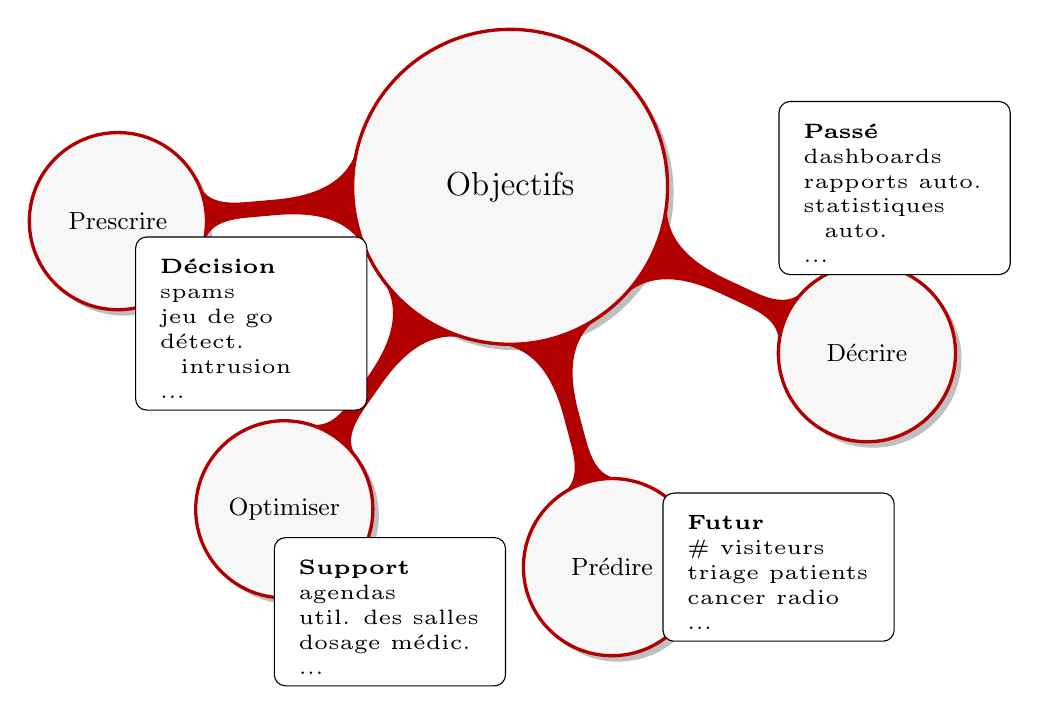
\begin{tikzpicture}[every annotation/.style = {draw, fill = white}]
		\tikzset{concept/.append style={fill={black!3},drop shadow}}
		\path[mindmap,concept color=red!70!black,text=black]
			node[concept] (objs) {Objectifs}
			[clockwise from=-25]
			child { node[concept] (dec) {Décrire} }
			child[sibling angle=50] { node[concept] (pred) {Prédire} }
			child[sibling angle=50] { node[concept] (opt) {Optimiser} }
			child[sibling angle=50] { node[concept] (pres) {Prescrire} }
		;
		\info{dec.north}{above,anchor=south,xshift=1em,yshift=-1em}{%
		\item[] \textbf{Passé}
		\item[] dashboards
		\item[] rapports auto.
		\item[] statistiques auto.
		\item[] ...
		}
		\info{pred.east}{above,anchor=west,xshift=-2em,yshift=0em}{%
		\item[] \textbf{Futur}
		\item[] \# visiteurs
		\item[] triage patients
		\item[] cancer radio
		\item[] ...
		}
		\info{opt.south}{above,anchor=west,xshift=-1em,yshift=-.5em}{%
		\item[] \textbf{Support}
		\item[] agendas
		\item[] util. des salles
		\item[] dosage médic.
		\item[] ...
		}
		\info{pres.south}{above,anchor=west,yshift=-.5em}{%
		\item[] \textbf{Décision}
		\item[] spams
		\item[] jeu de go
		\item[] détect. intrusion
		\item[] ...
		}
\end{tikzpicture}

\end{document}
